\subsection{Implementationsarkitektur}
Modell över implementationsarkitektur, koppling till motiveringen och diagram.

\subsubsection{Modell UI-Applikation}
Figur \ref{fig:implementationsarkitektur-UI} visar en modell över implementationsarkitekturen för UI-Applikationen. Kommunikationen från komponenten benämnd UI-kommunikation går till den IoT-Backend som presenteras i konceptarkitekturen.Denna är här utelämnad för tydlighet. Streckade rutor är grupperingar av komponenter som utgör stora delar i systemet. Gränssnittet mellan spel och spelläge ska betraktas som en viktig informationsväg och inte en självstående komponent.

\begin{figure}[h]
    \centering
    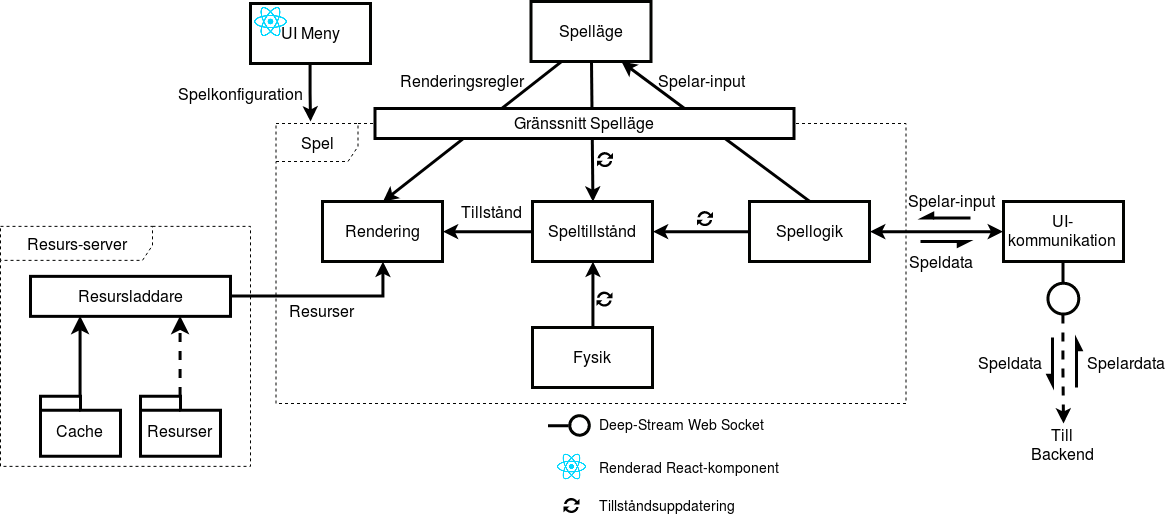
\includegraphics[scale=0.4]{implementationsarkitektur_UI}
    \caption{Modell över implementationsarkitektur för UI-Applikationen}
    \label{fig:implementationsarkitektur-UI}
\end{figure}

\subsubsection{Beskrivning UI-Applikation}

\subsubsection{Modell Kontroll-Applikation}
Implementationsarkitekturen för kontroll-applikationen presenteras i figur \ref{fig:implementationsarkitektur-kontroll}. Även denna följer samma notation som för UI-Applikationen. Resurs-servern är identisk med samma komponent i UI-delen.

\begin{figure}[h]
    \centering
    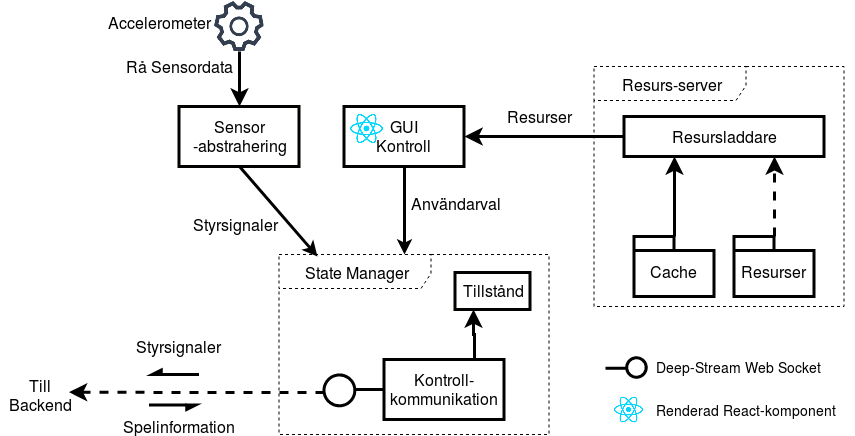
\includegraphics[scale=0.4]{implementationsarkitektur_kontroll}
    \caption{Modell över implementationsarkitektur för Kontroll-Applikationen}
    \label{fig:implementationsarkitektur-kontroll}
\end{figure}

\subsubsection{Beskrivning Kontroll-Applikation}
